% =========================================================================== %
% Preamble                                                                    %
% =========================================================================== %

\documentclass[dvipsnames, 12pt]{article}
\usepackage[utf8]{inputenc}

% Set paper geometry
\usepackage[letterpaper, margin=1.87cm]{geometry}

% Must include this before setting title and author
\usepackage{findlay}

\title{\huge Towards Adaptive Process Confinement
Mechanisms\\{\large COMP5900I Literature Review}}

\author{William Findlay}
% For acmart.cls:
%\affiliation{Carleton University}
%\email{williamfindlay@cmail.carleton.ca}

% Add bibliography:
\addbibresource{references.bib}

% To set sans serif font:
%\renewcommand{\familydefault}{\sfdefault}

\lhead{Towards Adaptive Process Confinement Mechanisms}

% Magic to stop overfull hbox in bibliography!
\emergencystretch=1em

\ExecuteBibliographyOptions{maxbibnames=999}

\setlist[enumerate]{
  leftmargin=*
}

% =========================================================================== %
% Document                                                                    %
% =========================================================================== %

\begin{document}

% Title page
\maketitle
\thispagestyle{empty}
%\pagenumbering{roman}
%\newpage

% Table of Contents, List of Figures, List of Tables, List of Listings
%\begingroup
%\hypersetup{linkcolor=black}
%\tableofcontents
%\newpage
%\listoffigures
%\newpage
%\listoftables
%\newpage
%\lstlistoflistings
%\newpage
%\endgroup

\vfill
\begin{abstract}
\todo{Come back hither when done.}
\end{abstract}
\vfill
\vfill

\clearpage

% Reset page numbering
\pagenumbering{arabic}
\setcounter{page}{1}

% Uncomment for 1.5 spacing:
%\onehalfspacing

\section{Introduction}
\label{sec:introduction}

Restricting unprivileged access to system resources has been a key focus of
operating systems security research since the inception of the earliest
timesharing computers in the late 1960s and early 1970s
\cite{graham1968_protection, ritchie1973_unix, corbato1962_ctss}. In its
earliest and simplest form, access control in operating systems meant preventing
one user from interfering with or reading the data of another user. The natural
choice for many of these early multi-user systems, such as Unix
\cite{ritchie1973_unix}, was to build access control solutions centred around
the user model---a design choice which has persisted in modern Unix-like
operating systems such as Linux, OpenBSD, FreeBSD, and MacOS.  Unfortunately,
while user-centric permissions offer at least some protection from other users,
they fail entirely to protect users from \textit{themselves} or from their own
\textit{processes}.  It was long ago recognized that finer granularity of
protection is required to truly restrict a process to its desired functionality
\cite{lampson1973_a_note}. This is often referred to as \textit{the process
confinement problem} or \textit{the sandboxing problem}.

Despite decades of work since Lampson's first proposal of the process
confinement problem in 1973 \cite{lampson1973_a_note}, it remains largely
unsolved to date \cite{crowell2013_confinement_problem}. This begs the question
as to whether our current techniques for process confinement are simply
inadequate for dealing with an evolving technical and adversarial landscape.  In
this literature review, I argue that, in order to solve the process confinement
problem, we need to rethink the status quo in process confinement, and instead
move towards \textit{adaptive} process confinement mechanisms.  Here, I define
adaptive process confinement mechanisms as those which greatly help defenders
confine their processes, are easily adoptable across a variety of system
configurations, and are robust in the presence of attacker innovation.  Roughly,
this definition can be broken down into the following properties:
\begin{enumerate}[label=\bfseries P\arabic*., ref=P\arabic*, labelindent=2em]
    \item \label{p:1} \textsc{High robustness to attacker innovation.} An adaptive
    process confinement mechanism should continue to protect the host system,
    even in the presence of attacker innovation. That is, it should be resistant
    to an adaptive adversary.

    \item \label{p:2} \textsc{Low adoption effort.} An adaptive process
    confinement mechanism should require minimal effort to adopt on a variety of
    system configurations. It should work out of the box on the majority of
    target systems and should be deployable in a production environment without
    major security or stability concerns.

    \item \label{p:3} \textsc{High reconfigurability.} An adaptive process
    confinement mechanism should be highly reconfigurable based on the needs of
    the end user and the environment in which it is running. This
    reconfiguration could either be automated, semi-automated, or manual, but
    should not impose significant adoptability barriers (c.f.~\ref{p:2}).

    \item \label{p:4} \textsc{High transparency.} An adaptive process
    confinement mechanism should be as transparent to the end user as possible.
    It should not get in the way of ordinary system functionality, and should
    not require the modification of application source code in order to
    function. Further, its base functionality should not require significant
    user intervention, if at all.

    \item \label{p:5} \textsc{High usability (by non-experts).} An adaptive process confinement
    mechanism should maximize its usability such that it is usable by largest
    and most diverse set of defenders possible. In particular, it should not
    require significant computer security expertise from its users.
\end{enumerate}

To argue the case for adaptive process confinement, we need to understand the
existing process confinement literature from an adaptive perspective. To that
end, I present a novel taxonomy of the existing literature, categorizing process
confinement mechanisms as either \textit{maladaptive} or \textit{semi-adaptive}.
In light of this categorization, I then discuss what the move toward
\textit{truly adaptive} process confinement mechanisms might look like.

%In this literature review, I present the status quo in process confinement,
%with an emphasis on Unix and modern Unix-like systems such as Linux.  Further,
%I present a novel taxonomy, categorizing existing process confinement
%mechanisms into \textit{maladaptive}, \textit{semi-adaptive}, and
%\textit{adaptive} solutions.  Finally, I argue the case for the development and
%adoption of \textit{adaptive process confinement mechanisms}.

The rest of this paper proceeds as follows. \Cref{sec:threat_model} presents the
process confinement threat model.
%and examines the motivation for considering
%process confinement from an adaptive security perspective.
\Cref{sec:maladaptive} discusses maladaptive process confinement solutions, while
\Cref{sec:semi-adaptive} presents semi-adaptive approaches that fail to meet the
mark of a truly adaptive process confinement mechanism. \Cref{sec:towards}
discusses moving toward truly adaptive process confinement mechanisms and argues
that new operating system technologies coupled with well-known techniques from
the anomaly detection literature may enable a paradigm shift in this direction.
\Cref{sec:conclusion} concludes.

\section{The Process Confinement Threat Model}
\label{sec:threat_model}

To understand why process confinement is a desirable goal in operating system
security, we must first identify the credible threats that process confinement
addresses. To that end, I first describe three attack vectors
(\crefrange{a:1}{a:3}), followed by three attack goals (\crefrange{g:1}{g:3})
which highlight just a few of the threats posed by unconfined processes to
system security, stability, and user privacy.

\begin{enumerate}[label=\bfseries A\arabic*., ref=A\arabic*, labelindent=2em]
    \item \label{a:1} \textsc{Compromised processes.} Unconfined running
    processes have classically presented a valuable target for attacker
    exploitation. With the advent of the Internet, web-facing processes which
    handle untrusted user input are especially vulnerable, particularly as they
    often run with heightened privileges \cite{cohen1996_secure}. An attacker
    may send specially crafted input to the target application, hoping to
    subvert its control flow integrity via a classic buffer overflow,
    return-oriented programming \cite{shacham2007_rop}, or some other means. The
    venerable Morris Worm, regarded as the first computer worm on the Internet,
    exploited a classic buffer overflow vulnerability in the \texttt{fingerd}
    service for Unix, as well as a development backdoor left in the
    \texttt{sendmail} daemon \cite{spafford1989_morris}. In both cases, proper
    process confinement would have eliminated the threat entirely by preventing
    the compromised programs from impacting the rest of the system.

    \item \label{a:2} \textsc{Semi-honest software.} Here, I define semi-honest
    software as that which appears to perform its desired functionality, but
    which additionally may perform some set of unwanted actions without the
    user's knowledge. Without putting a proper, external confinement mechanism
    in place to restrict the behaviour of such an application, it may continue
    to perform the undesired actions ad infinitum, so long as it remains
    installed on the host. As a topical example, an \texttt{strace} of the
    popular Discord \cite{discord} voice communication client on Linux reveals
    that it repeatedly scans the process tree and reports a list of \textit{all
    applications} running on the system, even when the \enquote{display active
    game} feature\footnote{This feature allows Discord to report, in the user's
    status message, what game the user is currently playing, and appears to be
    the original motivation behind scanning the process tree.} is turned off.
    This represents a clear violation of the user's privacy expectations.

    \item \label{a:3} \textsc{Malicious software.} In contrast to semi-honest
    software, malicious software is that which is expressly designed and
    distributed with malicious intent. Typically this software would be
    downloaded by an unsuspecting user either through social engineering
    (e.g.~fake antivirus scams) or without the user's knowledge (e.g.~a drive-by
    download attack). It would be useful to provide the user with a means of
    running such potentially untrustworthy applications in a sandbox so that
    they cannot damage the rest of the system.
\end{enumerate}

\begin{enumerate}[label=\bfseries G\arabic*., ref=G\arabic*, labelindent=2em]
    \item \label{g:1} \textsc{Installation of backdoors/rootkits.} Potentially
    the most dangerous attack goal in the exploitation of unconfined processes
    is the establishment of a backdoor on the target system.  A backdoor needn't
    be sophisticated---for example, installing the attacker's RSA public key in
    \texttt{ssh}'s list of authorized keys would be sufficient---however the
    most sophisticated backdoors may result in permanent and virtually
    undetectable escalation of privilege. For instance, a sophisticated attacker
    with sufficient privileges may load a \textit{rootkit}
    \cite{beegle2007_rootkit} into the operating system kernel, at which point
    she has free reign over the system in perpetuity (unless the rootkit is
    somehow removed or the operating system is reinstalled).

    \item \label{g:2} \textsc{Information leakage.} An obvious goal for attacks
    on unconfined processes (and indeed the focus of the earliest literature on
    process confinement \cite{lampson1973_a_note}) is information leakage. An
    adversary may attempt to gain access personal information or other sensitive
    data such as private keys, password hashes, or bank credentials. Depending
    on the type of information, an unauthorized party may not even necessarily
    require elevated privileges to access it---for instance, no special
    privileges are required to leak the list of processes running on a Linux
    system, as in the case of Discord \cite{discord} highlighted above.

    \item \label{g:3} \textsc{Denial of service.} A compromised process could be
    used to mount a denial of service attack against the host system. For
    example, an attacker could take down network interfaces, consume system
    resources, kill important processes, or cause the system to shut down or
    reboot at an inopportune moment.
\end{enumerate}

As shown in the examples above, unconfined processes can pose significant
threats to system security and stability as well as user privacy. With the
advent of the Internet, many of these threats are now exacerbated. Unconfined
network-facing daemons continually process untrusted user input, resulting in an
easy and potentially valuable target for attacker exploitation. Email and web
browsers have enabled powerful social engineering and drive-by download attacks
which often result in the installation of malicious software. Semi-honest
software can violate user expectations of security and privacy by performing
unwanted actions without the user's knowledge. It is clear that a solution is
needed to mitigate these threats---for this, we turn to process confinement.
Unfortunately, process confinement is not yet a solved problem
\cite{crowell2013_confinement_problem}, and so the exploration of new solutions
is necessary.

\section{Maladaptive Process Confinement Approaches}
\label{sec:maladaptive}

A \textit{maladaptive} process confinement mechanism is one which does not
cleanly fit the majority of the adaptive properties outlined in
\Cref{sec:introduction} (\crefrange{p:1}{p:5}). For example, a process
confinement mechanism with high reconfigurability and low adoption effort, but
with low robustness to attacker innovation, low transparency, and low usability
would constitute a maladaptive approach.

Unfortunately, maladaptive techniques cover the majority or the process
confinement literature, but many are widely used and studying them can provide
good insight into what an adaptive or semi-adaptive approach might do
differently in practice. To further compartmentalize this study, I categorize
maladaptive approaches into the lower-level techniques (i.e.~at the operating
system kernel or application source code levels) and the higher-level techniques
that often build upon them.

\subsection{Low Level Techniques}



\subsection{High Level Techniques}

In Linux, a recent trend of \textit{containerized package management} has emerged.

\begin{figure}[htpb]
    \centering
    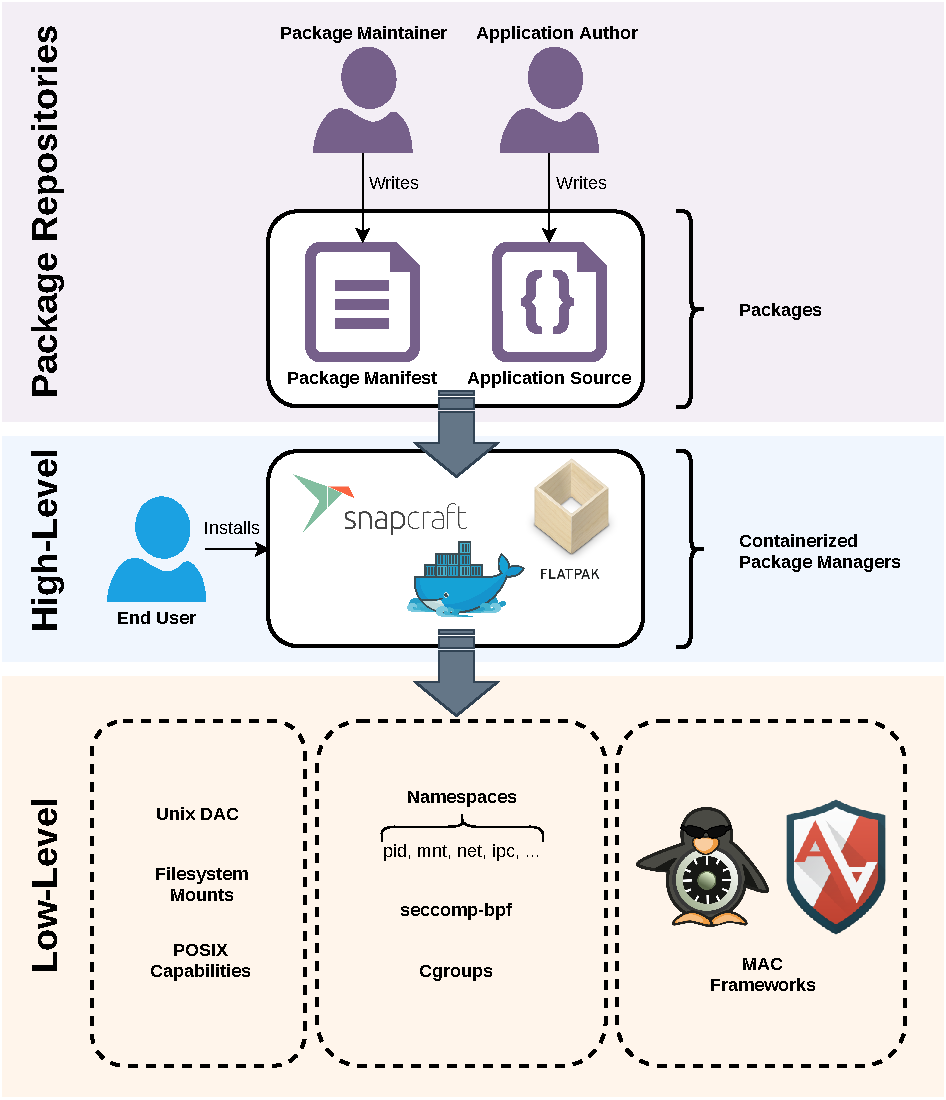
\includegraphics[width=0.6\linewidth]{figs/high-level.pdf}
    \caption{
        The basic architecture of containerized package management solutions for
        Linux, such as Snapcraft \cite{snap}, Flatpak \cite{flatpak}, and Docker
        \cite{docker}. Package maintainers write high-level, coarse-grained
        package manifests, which are then compiled into policy for lower-level
        process confinement mechanisms to enforce.
    }%
    \label{fig:containerized}
\end{figure}

\section{Semi-Adaptive Process Confinement Approaches}
\label{sec:semi-adaptive}

\subsection{Automated Policy Generation}

\subsection{Automated Policy Auditing}

\section{Towards Truly Adaptive Process Confinement}
\label{sec:towards}

\subsection{Anomaly Detection Techniques}

\subsection{Extended BPF}

\section{Conclusion}
\label{sec:conclusion}


% Uncomment for bibliography:
%\nocite{*} % TODO: Comment this out when done
\clearpage
\printbibliography

\end{document}

% vim:syn=tex
